% IEEE conference-format paper. Class: IEEEtran (conference option).
% Previous title of this draft: "From Headline to Currency Reaction: Predicting Affected Pairs,
% Direction, Magnitude and Confidence of FX Moves from News, for Ranking Arbitrage Opportunities".
% Research content: commit 639fcdf on branch semantic-microservice (research/artifacts/*.json and
% research/RESEARCH_TRACKER.md). Every number traces to an artifact or the tracker; see
% build_numbers.py (trace table) and check_paper.py (structure), both in this folder.
\documentclass[conference]{IEEEtran}
\IEEEoverridecommandlockouts
\usepackage{cite}
\usepackage{amsmath,amssymb}
\usepackage{graphicx}
\usepackage{booktabs}
\usepackage{adjustbox}
\usepackage{textcomp}
\usepackage[hidelinks]{hyperref}

\newcommand{\bps}{\,bps}

\begin{document}

\title{What News Can and Cannot Tell a Cross-Venue FX Arbitrage Detector: Pre-Registered Evidence on Direction, Move Size and Ranking}

% \authorbox{name}{role line}{email}
\newcommand{\authorbox}[3]{\begin{tabular}[t]{@{}c@{}}
#1\\ \textit{#2}\\ \textit{PES University}\\ Bangalore, India\\ #3
\end{tabular}}
\author{%
\authorbox{Dr. Chaitra B}{Associate Professor, Dept. of CSE}{chaitrab@pes.edu}%
\hspace{2.5em}%
\authorbox{Dhruv Menon}{Student, Dept. of CSE}{dhruvmenon2005@gmail.com}%
\hspace{2.5em}%
\authorbox{Davis Philip}{Student, Dept. of CSE}{dav.philip28@gmail.com}\\[2ex]
\authorbox{Nikhil Thomas Sojan}{Student, Dept. of CSE}{nikhil.thomas.sojan@gmail.com}%
\hspace{2.5em}%
\authorbox{Navika Srikanth}{Student, Dept. of CSE}{navikasrikanth@gmail.com}%
}

\maketitle

\begin{abstract}
A cross-venue foreign-exchange (FX) arbitrage detector finds crossed quotes but cannot tell which
of them news has made risky. We test what news can add: direction, move size and ranking. For
scheduled releases, a fixed theory rule gets the direction of the 15-minute reaction right 68.4\%
of the time (95\% interval 65.4 to 71.3, 1,385 releases) and a learned model 63.5\%. From the time
an article appears, the direction is gone: 48.8\% (46.6 to 51.0) at the registered 15-minute delay,
and an exploratory scan finds accuracy of 48.8 to 52.6\% at every delay from 1 to 30 minutes, none
significantly different from a coin ($p\ge0.055$). The
median effective article delay was 23 minutes over 9 measured releases. For unscheduled news,
direction is null, but headline activity predicts the size of the next move (coefficients 0.043 and
0.048), and the effect replicated on 18 new months (0.0405, $p=0.003$). An
exploratory control shows that 61 to 72\% of that coefficient is shared with the previous 24 hours'
volatility; a smaller effect survives (0.020 at 60 minutes, $p=0.0003$). In a live recording the
news channels gave no ranking gain and a news-as-risk test was not supported; the live sample is
small and partly contaminated. We report three silent data errors that each changed a conclusion,
with an internal pre-registration log and a reproducibility package.
\end{abstract}

\begin{IEEEkeywords}
foreign exchange, arbitrage, news analytics, event study, calibration, pre-registration,
data quality
\end{IEEEkeywords}

%--------------------------------------------------------------------------------------------
\section{Introduction}
A cross-venue arbitrage detector flags the moments when one venue's bid exceeds another venue's
ask. Once both legs fill, the position is close to market-neutral. What remains is execution
risk: legging exposure while the second leg is pending, and stale quotes around news.
Algorithmic traders in the FX market are known to remove triangular arbitrage
opportunities~\cite{chaboud2014}, so what is left for a detector is short-lived. A news layer is only useful to such a detector if it answers, for each
article and each pair, four questions. Is the pair affected? Which way does it move? By how
much? How sure is the answer? The last answer has to be a probability that means what it says,
because a ranker uses it as a weight.

We study these questions under a pre-registered protocol and report what we found, including the
results that went against our expectation. Our contributions are:
\begin{enumerate}
\item A pre-registered separation of what is predictable at the time of a scheduled release from
what is predictable when an article about it arrives, with the article delay measured on live
feeds and an exploratory scan showing no direction distinguishable from chance for any delay of one minute or more
(Sections~\ref{sec:sched} and~\ref{sec:live}).
\item Evidence that news \emph{activity} predicts the size of the next move, replicated out of
sample, but with most of the coefficient shared with the previous 24 hours' volatility and a
smaller effect surviving the control, while direction and novelty fail; the novelty hypothesis (H1)
was significant with the wrong sign and is reported as such (Section~\ref{sec:unsched}).
\item Live ranking tests (H6b, RQ5, C40, C43 and prospective scoring) that find no ranking value
for the news channels, with their limits stated (Section~\ref{sec:live}).
\item Three silent errors in free FX and news data, each shown to change a result, and a
reproducibility package (Sections~\ref{sec:data} and~\ref{sec:repro}).
\end{enumerate}

\section{Related Work}
High-frequency FX responses to macroeconomic announcements are documented by
Andersen et al.~\cite{abdv2003}, Faust et al.~\cite{faust2007} and Evans and
Lyons~\cite{evanslyons2008}: surprises move exchange rates within minutes, with signs that follow
economic priors, and volatility stays elevated for roughly fifteen minutes afterwards~\cite{ederington1993}. Our
scheduled-release study replicates this on corrected data and turns it into an article-level
predictor. Tetlock~\cite{tetlock2011} studies whether investors react to stale information, which
motivates our novelty hypothesis, and Gro{\ss}-Klu{\ss}mann and Hautsch~\cite{grossklussmann2011}
quantify news-implied reactions with automated text analytics. Baker et al.~\cite{bbd2016} build
news-based indices of the kind our currency-level factor follows. Sentiment baselines use
FinBERT~\cite{araci2019}, novelty uses sentence embeddings~\cite{reimers2019}, and unscheduled
news comes from GDELT~\cite{leetaru2013}. Inference follows cluster-robust
practice~\cite{cameronmiller2015} with false-discovery control~\cite{bh1995}; intervals are
split-conformal~\cite{lei2018}; calibration is measured as in~\cite{guo2017}. The study follows
the pre-registration idea~\cite{nosek2018} with an internal log rather than an external registry
(Section~\ref{sec:method}).

%--------------------------------------------------------------------------------------------
\section{Data and Three Silent Errors}\label{sec:data}
\subsection{Sources}
\emph{Scheduled releases.} A ForexFactory-format calendar dump (34,333 events, 2018-01 to
2025-04; 23,636 with a usable time and 22,517 with a standardized surprise). Surprises are
standardized per (currency, indicator) by a $\sigma$ estimated outside 2020-03-01..2021-06-30 and
winsorized at $\pm5\sigma$. Prices are HistData one-minute bid bars for EUR/USD, GBP/USD, USD/JPY
and USD/CHF. The release study uses 1,385 high-impact, exact-time releases with $z\neq0$ (USD,
EUR, GBP, JPY, CHF), each paired with the four majors.

\emph{Unscheduled news.} FX-term headlines from the GDELT Global Knowledge Graph (3,690,637
extracted, 1,576,465 currency-tagged). The frozen sample covers 2019-10 to 2025-04 (67 months,
1,569,940 events; 955,570 canonical headlines after de-duplication) and is scored with a lexicon,
FinBERT and a sentence-transformer. A second sample of 18 months (2025-05 to 2026-10; 399,810
tagged events, 250,509 canonical) is used only for the replication in Section~\ref{sec:unsched}.

\emph{Live data.} A recorder logged 37,604 cross-venue opportunities from 25~Oct to 6~Nov 2026,
each with a snapshot of every news channel. The venues are Kraken and TrueFX, an indicative
aggregated feed; detected crosses are therefore price discrepancies, not executable arbitrage.

\subsection{Error 1: calendar timestamps}
About 30\% of calendar rows store a missing time as local midnight, including all 88 payrolls
releases of 2018--2025, and the dump's UTC offsets keep a daylight-saving rule that no longer
applies (5,071 rows from 2023 onward were one hour early). Our pre-registered positive control
failed twice on these clocks. On corrected clocks the original specification passes all three
criteria (payrolls 5-minute EUR/USD $\beta=-8.99$\bps/$\sigma$, $p=0.010$; pooled
$+6.51$, $p\approx10^{-11}$; placebo $p=0.33$). The pre-registered record remains a failure; the
pass is post hoc, and the fixes were made from documentation and observed rows, never from prices.

\subsection{Error 2: daylight saving in price files}
The one-minute files described as fixed Eastern Standard Time are New York wall-clock time with
daylight saving. The symptom was a reaction ``jump'' exactly 60 minutes after every summer
release. The summer one-minute reaction is $+0.5$\bps{} on the documented clock and $+8.5$\bps{}
after the fix, so the first H2/H3 pass was void.

\subsection{Error 3: news API truncation}
A 24-hour GDELT DOC request with newest-first sorting and a 250-record cap returns only the
minutes before midnight UTC (Fig.~\ref{fig:gdelt}). In a 169-day sample 88\% of kept headlines
fall between 23:00 and 01:00 UTC, and the median daily span is 0.2~h. We withdrew the daily
sample and re-collected news from the GDELT Global Knowledge Graph, where page titles exist only
from September 2019. A rule that treated the 20 empty earlier months as ``no FX news'' would have
been wrong, so the sample starts in 2019-10 (Appendix~\ref{app:dev}, D5).

\subsection{Further contamination in the live pipeline}
The live feed filled quiet periods with synthetic demo headlines. These made up 13,311 of the
14,486 logged predictions (92\%) before 2~Nov and 190 of 743 USD/INR training rows of an earlier
text model, which voids that model's USD/INR metrics. They are excluded from every analysis.
The live window also ran on a keyword scorer until FinBERT was enabled on 5~Nov, and a reconnect
storm on 3~Nov produced 8,355 repeated prediction rows; both are handled as sensitivity
sections.

\begin{figure}[t]\centering
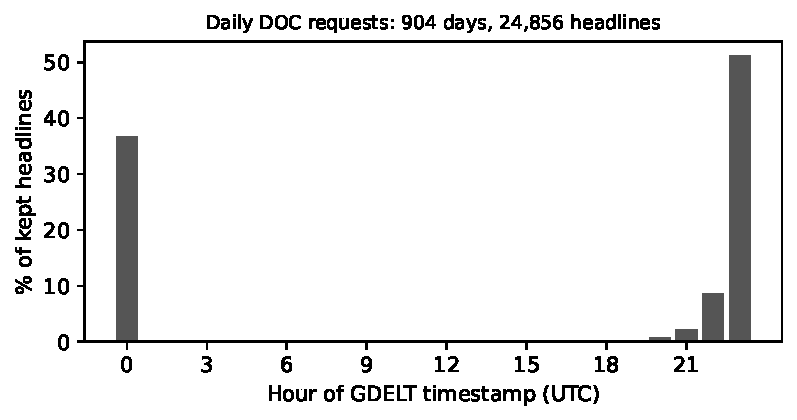
\includegraphics[width=0.85\columnwidth]{figures/gdelt_daily_defect.pdf}
\caption{Time of day of headlines kept by daily GDELT DOC requests: 88\% are stamped between
23:00 and 01:00 UTC.}\label{fig:gdelt}
\end{figure}

%--------------------------------------------------------------------------------------------
\section{Pre-Registration and Method}\label{sec:method}
Hypotheses, metrics, baselines and stop rules were fixed in a dated, append-only, version-controlled
protocol log before results; it is not an external registry, so its timing can be verified only
from the repository history. Every departure is a numbered deviation made before the affected
result existed (Appendix~\ref{app:dev}). Negative results are reported, and no test was
re-specified after its result was seen.

\subsection{Units and targets}
The unit is a release $\times$ pair. Release-time returns $r(0,h)$ use
$h\in\{1,5,15,30,60,120\}$ minutes, with 15 as primary. Because an article reporting a release
appears after it, we also measure arrival-time returns $r(15,15{+}h)$ with $h\in\{15,45,105\}$;
the primary window is 15--60 minutes. Returns are log returns in basis points between the first
bars at or after the window ends (bars stamped at close; entry lag $\le2$ minutes, exit lag
$\le5$ minutes, otherwise dropped).

\subsection{Model}
Direction is $\hat s=\operatorname{sign}(\hat\beta z)$, with $\hat\beta$ fitted through the origin
per (release currency, category, pair). The a-priori comparison is the theory rule
$\operatorname{sign}(z)\times$ (the indicator's economic sign). The expected move is
$|r|=a+b|z|+c\,v$, where $v$ is the same-clock mean absolute return over the previous 20
weekdays. Confidence is $P(\hat s\text{ correct}\mid|z|)$ from logistic regression, and
move-size intervals are split-conformal. An expanding monthly walk-forward with 12 training-only
months gives 76 test months (2019-01 to 2025-04). Inference is clustered by release moment
(about 900 clusters); for the unscheduled-news regressions it is clustered by UTC date.

\subsection{Deployed system}
A semantic microservice (V2) matches a headline to a calendar release, extracts the actual
figure, computes $z$ and returns per-pair direction, a calibrated probability and an expected move.
A currency index gives a per-currency news bias (FinBERT polarity $\times$ confidence $\times$
novelty $\times$ relevance, 12-hour decay); the pair bias is base minus quote. A risk channel
penalizes a pair when the expected move is large relative to its 24-hour median or a high-impact
release is within $-15$ to $+10$ minutes; a direction channel penalizes a trade when the index
opposes its residual exposure.

%--------------------------------------------------------------------------------------------
\section{Results: Scheduled Releases}\label{sec:sched}

\subsection{Direction (RQ2)}
Table~\ref{tab:dir} shows the release reaction is predictable: 75.2\% at one minute and 68.4\% at
15 minutes for the theory rule. The learned model does not beat the theory rule: its point
estimate is lower at every window, the intervals at the primary window overlap, and we ran no
paired test. The two agree on 82\% of rows. Accuracy rises with $|z|$ (58\%, 65\%, 68\% across
terciles). From article arrival the learned model's direction is at chance: 48.8\% for the
primary window ($p=0.27$).

\begin{table}[t]\centering\footnotesize
\caption{Out-of-sample direction accuracy (\%). $^\dagger$ primary. 95\% intervals are clustered by
release moment.}\label{tab:dir}
\begin{adjustbox}{max width=\columnwidth}
\begin{tabular}{@{}lrrr@{}}
\toprule
Window (min) & Learned model & Theory rule & Majority\\
\midrule
release 0--1 & 68.2 & 75.2 & 51.5\\
release 0--15$^\dagger$ & 63.5 [60.2, 66.6] & 68.4 [65.4, 71.3] & 51.5\\
release 0--60 & 60.4 & 64.4 & 51.8\\
release 0--120 & 57.7 & 61.0 & 52.2\\
\midrule
arrival 15--30 & 47.9 & 50.5 & 51.5\\
arrival 15--60$^\dagger$ & 48.8 [46.6, 51.0] & 51.0 [48.0, 53.7] & 50.5\\
arrival 15--120 & 50.2 & 50.1 & 49.7\\
\bottomrule
\end{tabular}
\end{adjustbox}
\end{table}

\subsubsection{How fast the move happens, and how late the article is}
The registered arrival window starts 15 minutes after the release, so we also ran an exploratory
scan of the assumed article delay $d$ (C47): the learned model's direction on the window
$r(d,d{+}45)$ for $d\in\{0,1,2,5,10,15,30\}$ minutes, with offsets fixed before the run and no
correction for seven offsets (Table~\ref{tab:decay}, Fig.~\ref{fig:decay}a). At $d=0$, the release
reaction itself, accuracy is 62.3\% and the mean move in the predicted direction is 8.49\bps. From
one minute on, accuracy is between 48.8\% and 52.6\% and the directed move between $-0.14$ and
$+0.73$\bps{} (all $p\ge0.19$). The 5-minute 52.6\% ($p=0.055$; interval 50.1 to 55.2) is one of seven tests and we do
not read it as a signal. Offset 15 reproduces the registered primary (48.8\%). So the move is in the
price within the first minute, and the arrival result does not depend on the 15-minute assumption.

\begin{table}[t]\centering\footnotesize
\caption{Exploratory scan of the assumed article delay $d$ (min): model direction accuracy on
$r(d,d{+}45)$ with $p$ against a coin, and mean move in the predicted direction (bps) with its $p$.
Seven offsets, no correction; $d=0$ is the release reaction.}\label{tab:decay}
\begin{adjustbox}{max width=\columnwidth}
\begin{tabular}{@{}lrrrrrrr@{}}
\toprule
$d$ (min) & 0 & 1 & 2 & 5 & 10 & 15 & 30\\
\midrule
Accuracy (\%) & 62.3 & 51.4 & 52.1 & 52.6 & 49.9 & 48.8 & 50.0\\
$p$ & $3.3\times10^{-15}$ & 0.27 & 0.10 & 0.055 & 0.91 & 0.27 & 0.98\\
Move (bps) & +8.49 & +0.23 & +0.58 & +0.73 & +0.09 & $-0.14$ & $-0.03$\\
$p$ & $4.6\times10^{-11}$ & 0.71 & 0.32 & 0.19 & 0.84 & 0.68 & 0.94\\
\bottomrule
\end{tabular}
\end{adjustbox}
\end{table}

Fewer than half of the articles arrive within 15 minutes. Over 19 article--feed rows for 9 releases, the
median delay from release to our first receipt was 37.5 minutes per row and 23.1 minutes per
release for the first article to arrive (effective latency; quartiles 6.7 and 37.5), and 44\% of
releases had an article within 15 minutes (Fig.~\ref{fig:decay}b). The latency study could match
only 2 of 10 high-impact calendar events, so its coverage is 20\%, and with fewer than 10 releases
it did not estimate an offset, so the 15-minute assumption stands, and the scan above shows the
result does not need it.

\begin{figure}[t]\centering
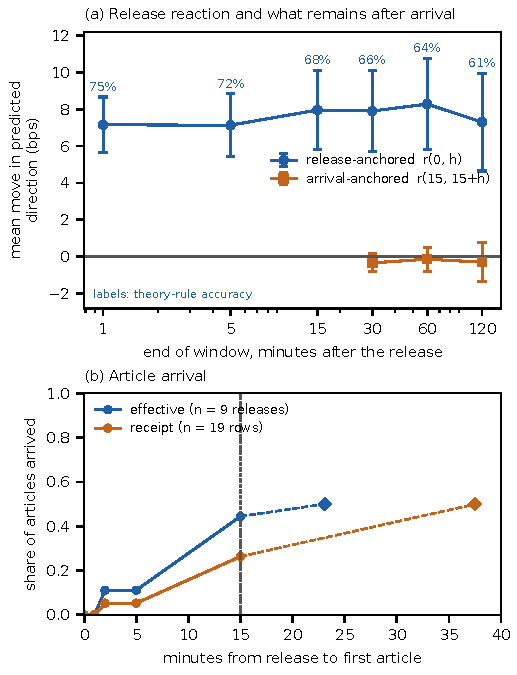
\includegraphics[width=\columnwidth]{figures/decay.pdf}
\caption{(a) Direction accuracy of the learned model with 95\% intervals against the assumed
article delay (diamond: the release reaction at $d=0$; dashed line: chance; exploratory). (b) Share of articles arrived within
1, 2, 5 and 15 minutes of the release (solid). The dashed segment joins the 15-minute share to the
median (diamond); the delay between them was not observed.}\label{fig:decay}
\end{figure}

\subsection{Magnitude (RQ3)}
The model ranks moves better than the training-mean baselines (Spearman 0.29 against 0.19 and 0.24
at 15 minutes) but its mean absolute error is not lower (12.01 against 11.54\bps{}, difference
$+0.47$, $p=0.15$). After arrival the same-clock volatility baseline beats it (7.11 against
7.40\bps, $p<0.001$), as Table~\ref{tab:mag} shows.

\begin{table}[t]\centering\footnotesize
\caption{Magnitude: MAE (bps) / Spearman $\rho$ out of sample.}\label{tab:mag}
\begin{adjustbox}{max width=\columnwidth}
\begin{tabular}{@{}lrrrr@{}}
\toprule
Window & Model & Pair mean & Cell mean & Same-clock $v$\\
\midrule
release 0--15$^\dagger$ & 12.01 / 0.29 & 11.54 / 0.19 & 11.59 / 0.24 & 11.85 / 0.29\\
arrival 15--60$^\dagger$ & 7.40 / 0.16 & 7.27 / 0.07 & 7.43 / 0.08 & \textbf{7.11} / 0.22\\
\bottomrule
\end{tabular}
\end{adjustbox}
\end{table}

\subsection{Confidence (RQ4)}
The confidence output is calibrated but resolves little (Table~\ref{tab:conf},
Fig.~\ref{fig:rel}). At 15 minutes the expected calibration error is 0.041 and the Brier score
0.234 against 0.232 for a constant rate; at one minute it beats the constant (0.207 against
0.217). Conformal intervals cover 76.5\% and 86.9\% at nominal 80\% and 90\%.

\begin{table}[t]\centering\footnotesize
\caption{Calibration and conformal coverage.}\label{tab:conf}
\begin{adjustbox}{max width=\columnwidth}
\begin{tabular}{@{}lrrrrr@{}}
\toprule
Window & ECE & Brier & Const. & Cov.\ 80\% & Cov.\ 90\%\\
\midrule
release 0--1 & 0.042 & 0.207 & 0.217 & 76.8 & 87.0\\
release 0--15$^\dagger$ & 0.041 & 0.234 & 0.232 & 76.5 & 86.9\\
arrival 15--60$^\dagger$ & 0.056 & 0.259 & 0.250 & 78.5 & 89.1\\
\bottomrule
\end{tabular}
\end{adjustbox}
\end{table}

\begin{figure}[t]\centering
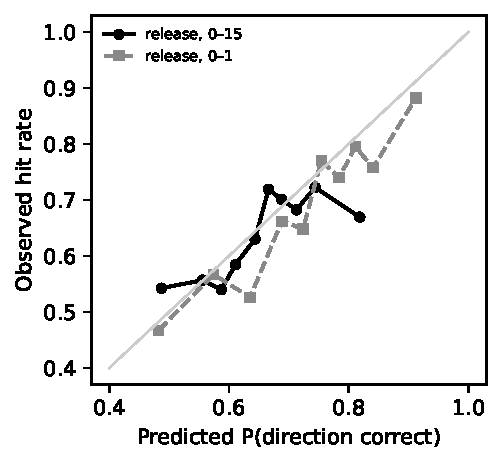
\includegraphics[width=0.55\columnwidth]{figures/reliability.pdf}
\caption{Reliability of the confidence output (equal-mass bins).}\label{fig:rel}
\end{figure}

\subsection{Affected pairs (RQ1) and categories}
The currency rule (a pair is affected if it contains the release currency) recalls 90\% of
abnormal moves at 41\% precision (F1 0.56). A move is abnormal for 41\% of own-pair rows but
19\% of cross-pair rows, so a euro-area release moves GBP/USD and USD/JPY abnormally about 22\%
of the time. Releases from JPY and CHF are too few for currency-level estimates, and none is
reported. Categories differ in size, not speed (Table~\ref{tab:h2}): inflation exceeds
employment, which exceeds growth, all within a minute and persistent to 120 minutes. The
half-life of a reaction is undefined in 98--100\% of bootstrap draws, so reaction speed by
category (H3) is not supported.

\begin{table}[t]\centering\footnotesize
\caption{Sign-oriented cumulative response (bps), US releases, four majors pooled. $^{*}$
survives Benjamini--Hochberg at $q\le0.05$.}\label{tab:h2}
\begin{adjustbox}{max width=\columnwidth}
\begin{tabular}{@{}lrrrrr@{}}
\toprule
Category & 1 min & 15 min & 60 min & 120 min & Dates\\
\midrule
inflation & 17.3$^{*}$ & 19.1$^{*}$ & 20.9$^{*}$ & 20.6$^{*}$ & 132\\
employment & 7.6$^{*}$ & 7.7$^{*}$ & 8.4$^{*}$ & 8.3$^{*}$ & 256\\
growth & 5.4$^{*}$ & 5.6$^{*}$ & 5.9$^{*}$ & 4.9$^{*}$ & 336\\
\bottomrule
\end{tabular}
\end{adjustbox}
\end{table}

%--------------------------------------------------------------------------------------------
\section{Results: Unscheduled News}\label{sec:unsched}
Each test below is one pass with its decision rule fixed beforehand. Multiplicity corrections and
every $p$-value are listed in the supplementary archive (\texttt{tables/pledger.tex}), except those
of the two exploratory checks of Tables~\ref{tab:decay} and~\ref{tab:volctl}.

\emph{H1, novelty and move size (not supported).} On 243,360 rows (234,273 events, 1,717 dates),
semantic novelty has a coefficient that is significant in the wrong direction ($\beta=-0.968$, SE
0.279, $p=0.0005$); out-of-sample MSE improves by 0.01\% (89.0017 to 88.9892), and we claim no
predictive value. The lexicon baseline agrees ($\beta=-0.937$, $p=0.0007$). The USD/INR arm
(101,176 events) is not significant ($\beta=-10.4$, $p=0.54$).

\emph{H5, sentiment as a currency factor (partial).} The lexicon passes the out-of-sample test
(R$^2$ 0.0073 against $-0.0006$; Spearman 0.123 against $-0.045$; loss-difference $p=0.003$) but
fails the market-component test: VIX $p=0.14$, USD/JPY $p=0.80$, USD/CHF with the wrong sign
($p=0.002$). FinBERT fails the out-of-sample test and passes only the VIX component
($p=0.026$).

\emph{H6, currency bias forecasts returns (not supported).} On 5,006 daily rows over 1,455 dates,
the pair-bias coefficient is $0.095$ ($p=0.89$), out-of-sample MSE is 2,270.5 against 2,268.4,
the hit rate is 49.4\% and rank ICs are $-0.02$ to $-0.03$.

\emph{Real release headlines (RQ2-E2E).} Of 2,410 candidate headlines (535 release moments) only
6.6\% match a calendar release and 4.7\% carry the correct actual figure. No method beats 50\% at
article time: structured 41.6\%, FinBERT 51.6\% [48.5, 54.4], the earlier text model 53.5\%
[49.1, 57.7].

\subsection{Thirty-minute window: direction and activity}
Per major pair and signal time $t$ (weekdays, every 30 minutes, 2019-10 to 2025-04), the news
window is the 30 minutes $(t-45,t-15]$ before the signal, lagged 15 minutes for GDELT's batch
clock. \emph{Activity} is the number of headlines in that window naming the base or the quote
currency. The \emph{abnormal move} over the next $h$ minutes is $|r|$ divided by the median $|r|$
at the same clock time on the previous 20 weekdays (at least 10 days). Test T2 regresses the log
abnormal move on $\log(1+\text{activity})$, a flag for a high-impact release of either currency in
the window, and pair dummies; standard errors are clustered by UTC date (1,445 clusters). T1
(direction) and T3 (caution) are rank-IC tests. Six tests, corrected together by Benjamini--Hochberg.

Direction is null (hit rate 50.0\%, $p=0.95$ at 30 minutes and $0.74$ at 60). Activity predicts
the size of the next move: the coefficients are 0.043 at 30 minutes ($q=6.1\times10^{-9}$) and
0.048 at 60 minutes ($q=1.5\times10^{-10}$), on 258,237 and 259,081 rows. A 10\% rise in
$1+$activity goes with an abnormal move about 0.4\% larger. A caution score is weakly predictive
at 60 minutes ($q=0.044$).

This result is net of the same-clock baseline and of a release flag, and in the replication below
of scheduled-release clocks. Busy news and an already volatile market could produce the same
pattern, so we ran a volatility control afterwards (below).

\subsection{Volatility control (C46, exploratory)}
Registered beforehand (C46), with no decision weight and reported as found, the control
re-estimates T2 on the rows that have both controls (224,495 rows and 1,439 dates at 60
minutes; 223,676 and 1,426 at 30), adding the abnormal move already under way inside the news
window (\emph{prior}), the pair's mean absolute return over the previous 24 hours relative to its
same-clock norm (\emph{level}), and both; the controls use returns that end before the signal.
Table~\ref{tab:volctl} gives the result. The prior move takes up 9 to 10\% of the coefficient;
the trailing level takes up 61\% at 60 minutes and 70\% at 30, and 63\% and 72\% with both. A
smaller effect survives both controls and stays significant: 0.020 ($p=0.0003$) at 60 minutes and
0.014 ($p=0.007$) at 30. We therefore read activity as partly a volatility-regime indicator (news
is busier on volatile days) that still carries a smaller signal about the next move's size, and we
do not claim that headlines cause larger moves. The base coefficient differs from 0.048 above
because it is estimated only on rows with both controls. The controls were not run on the
replication sample below, so we do not know how much of that effect survives them.

\begin{table}[t]\centering\footnotesize
\caption{Activity coefficient $\beta$ on $\log(1+\text{activity})$ with volatility controls,
$p$ clustered by UTC date, and shrinkage $1-\beta/\beta_{\text{base}}$ (\%).}\label{tab:volctl}
\begin{adjustbox}{max width=\columnwidth}
\begin{tabular}{@{}lrrrrrr@{}}
\toprule
 & \multicolumn{3}{c}{60 min} & \multicolumn{3}{c}{30 min}\\
Model & $\beta$ & $p$ & Shrink. & $\beta$ & $p$ & Shrink.\\
\midrule
Base & 0.0544 & $2.8\times10^{-12}$ & -- & 0.0489 & $1.4\times10^{-10}$ & --\\
+ prior & 0.0498 & $1.3\times10^{-11}$ & 8.6 & 0.0438 & $8.4\times10^{-10}$ & 10.4\\
+ level & 0.0213 & $2.1\times10^{-4}$ & 60.9 & 0.0148 & 0.0050 & 69.8\\
+ both & 0.0204 & $3.0\times10^{-4}$ & 62.6 & 0.0137 & 0.0074 & 71.9\\
\bottomrule
\end{tabular}
\end{adjustbox}
\end{table}

\subsection{Out-of-sample replication (C45)}
The activity result was the study's main positive finding, so before any new data was extracted we
registered a replication on the 18 months after the frozen sample (2025-05 to 2026-10; 40,196
and 34,556 rows; 370 UTC dates). The calendar dump ends in April 2025, so the release flag cannot
be built. The registered test (T2-clock) instead keeps only signal times with no scheduled-release
clock for either currency in $(t-45\text{ min},t+h]$, with clocks derived from the old sample
before extraction, and drops the release flag. Table~\ref{tab:c45} shows the replication: the
60-minute coefficient is 0.0405 ($p=0.003$), which meets the registered rule, and its size is close
to the original. The two specifications differ, and a like-for-like rerun of T2-clock on the
original sample is not reported. The volatility controls above were not run on this sample.
Direction is null again (rank IC $-0.008$ and $-0.005$; hit rates
49.4\% and 49.8\%), and the weak caution result at 60 minutes does not replicate (IC 0.000,
$p=1.00$). The notebook's optional FinBERT cell ran before the T2 output was read, so T1 and T3
were on screen at the same time as T2; T2 was computed first and did not change.

\begin{table}[t]\centering\footnotesize
\caption{News activity and the size of the next move: coefficient on $\log(1+\text{activity})$, SEs
clustered by UTC date. $^\dagger$ registered decision.}\label{tab:c45}
\begin{adjustbox}{max width=\columnwidth}
\begin{tabular}{@{}llrrrrr@{}}
\toprule
Sample & Min & Rows & Dates & $\beta$ & SE & $p$\\
\midrule
2019-10..2025-04 & 30 & 258,237 & 1,445 & 0.0427 & 0.0071 & $2.0\times10^{-9}$\\
 & 60 & 259,081 & 1,445 & 0.0481 & 0.0071 & $2.4\times10^{-11}$\\
2025-05..2026-10 (C45) & 30 & 40,196 & 370 & 0.0440 & 0.0119 & $2.4\times10^{-4}$\\
 & 60$^\dagger$ & 34,556 & 370 & 0.0405 & 0.0136 & 0.0030\\
\bottomrule
\end{tabular}
\end{adjustbox}
\end{table}

%--------------------------------------------------------------------------------------------
\section{Live Checks}\label{sec:live}
These checks use a small recording, and several are descriptive only. They do not show that the
news channels help, and they do not show that they are harmful in general.

\subsection{Setup and coverage}
The detector passes each opportunity through the news channels, which are logged as a snapshot.
The live ranker applied no semantic adjustment during the sample: the recorded score is the raw
detector score and every channel is shadow-logged, so detector-only comparisons are clean. In the
first eight analyses after the 5~Nov deployment the median total analysis time was 90\,ms.

The last quote was recorded at 01:19:47 IST on 7~Nov 2026, and about 10.9 days of the registered
window (to 18~Nov 00:00 IST) were never recorded. Appendix~\ref{app:downtime} lists every logged
outage; no gap was filled or worked around. A separate cloud recording began on 21~Nov; it is a
new sample and is not used here.

\subsection{Prospective scoring of the deployed models}
Rows are counted once per headline and pair, scored against the hour after receipt, and clustered
by UTC date (Table~\ref{tab:prosp}). The V1 text model scored 44.4\% on 124 scored rows, with 4
date clusters; the interval spans most of the unit range, so this is a description and not a test.
The V2.0 release model scored 61.5\% on 26 rows from 3 date clusters ($p=0.55$ against a coin).
The V2.1 release model got 21 of 23 rows right, but those rows are 12 distinct headlines about 4
releases over 2 days (a Bank of England decision, jobless claims, payrolls and consumer sentiment),
and each US release fans out to five pairs. We count this as 4 events and make no claim about live
accuracy; the interval the script reports comes from resampling 2 days and is not valid. This
sits alongside the pooled arrival result of Section~\ref{sec:sched} (48.8\% on about 3.5 thousand
rows), which stands: four large surprises cannot overturn it. Live expected calibration error was 0.22
to 0.30 for all three models.

\begin{table}[t]\centering\footnotesize
\caption{Prospective scoring of deployed models. Accuracy is the share of correct signs; the interval
is a date-clustered bootstrap.}\label{tab:prosp}
\begin{adjustbox}{max width=\columnwidth}
\begin{tabular}{@{}lrrrrrr@{}}
\toprule
Model & Rows & Scored & Dates & Accuracy & IC & ECE\\
\midrule
V1 text & 203 & 124 & 4 & 44.4 [10.8, 81.4] & $-0.36$ & 0.23\\
V2.0 release & 26 & 26 & 3 & 61.5 [16.7, 100] & $-0.11$ & 0.30\\
V2.1 release & 26 & 23 & 2 & 21 of 23 (4 events) & 0.57 & 0.22\\
\bottomrule
\end{tabular}
\end{adjustbox}
\end{table}

\subsection{H6b and RQ5: ranking value}
The outcome is whether the cross is still present at the next poll of both legs. Table~\ref{tab:h6b}
gives the area under the ROC curve (AUC), with a day bootstrap, for the detector alone and with
each channel added cumulatively. In H6b the risk and direction channels slightly lower the AUC (by
0.003 to 0.012); the window channels are indistinguishable from the detector. The realised edge at
the next poll is a mean of 2.3--2.4 pips (median 1.8--1.9). Most crosses persist (97.8--98.3\%), so
each H6b AUC rests on 448 to 790 negatives. The RQ5 extension covers the 916 opportunities after
the H6b window, from 3 days, with 42 negatives and a mean edge of 3.07 pips; on the updated
engine every interval for a difference from the detector contains zero. Four to six recorded
days give a coarse bootstrap, and the counts of rows overstate the independent information.

\begin{table}[t]\centering\footnotesize
\caption{Next-poll persistence ranking, AUC. Difference to detector in brackets (95\% day
bootstrap).}\label{tab:h6b}
\begin{adjustbox}{max width=\columnwidth}
\begin{tabular}{@{}lrrrr@{}}
\toprule
Sample (rows / days) & Detector & + risk & + risk + dir. & + window\\
\midrule
H6b locked (36,668 / 6) & 0.918 & 0.908 [$-.016,-.003$] & 0.906 [$-.017,-.004$] & 0.920 [$-.002,+.004$]\\
H6b clean (29,456 / 4) & 0.948 & 0.942 [$-.011,-.001$] & 0.941 [$-.012,-.001$] & 0.949 [$-.004,+.002$]\\
RQ5 (916 / 3) & 0.815 & 0.827 [$-.027,+.022$] & 0.827 [$-.027,+.022$] & 0.814 [$-.002,+.013$]\\
\bottomrule
\end{tabular}
\end{adjustbox}
\end{table}

\subsection{C40: news as risk (not supported)}
The pre-registered test asked whether crosses in release windows vanish more often than in matched
control windows, with a feed-quality check and an activity check, all three tests corrected together. The primary comparison (C40-1) could not be
computed: the live calendar archive held one week, so no control window was usable, and only 3
windows with opportunities exist against 30 required. We found this when the test ran; the archive
had been checked for format and not for how many weeks it held. The feed-quality check (C40-2,
age of the older quote) gave an AUC for ``not still crossed'' of 0.495 [0.462, 0.551]. The activity
check (C40-3) gave 0.531 [0.425, 0.552] on 30,351 opportunities over 6 days ($q=0.44$). Under the
registered rule, news as risk is \emph{not supported} on the live recorder. It is a non-confirmation
and not a refutation: the outcome is whether an indicative price gap survives about a second, the
sample is 8 days on a degraded venue, and the primary test could not be computed. One subset
(the RQ5 extension period) had an AUC of 0.551 with $p=0.0005$ on 914 rows and 42 vanished crosses,
one of several reported subsets, and we give it no weight.

\subsection{C43: shadow engine (exploratory)}
The shadow engine recorded 318 rows over 2 days, with 18 not still crossed. The risk-adjusted score
had an AUC of 0.863 against 0.844 for the detector; the interval for the difference resamples two
days and is not valid. The FX-relevance filter removed 83\% of the window's items (998 of 1,200
item slots over 221 rows with items), and the two window readings agreed on 88\% of rows, almost
all because both were neutral. We give this analysis no decision weight.

%--------------------------------------------------------------------------------------------
\section{Discussion}
For a ranker, the direction an article reports describes a move that has already happened: the
reaction is in the price within a minute, direction is at chance for any article delay of one
minute or more, and fewer than half of the first articles arrive within 15. The value of news may
lie elsewhere: in naming which venue's quote is stale, and in flagging a release window as
execution risk. News activity predicts how large the next move is, in two independent samples, but
most of that coefficient is shared with the previous day's volatility; direction does not survive
at any horizon we tested.

That risk reading did not carry over to the live recorder. The risk channel did not improve
next-poll persistence ranking in H6b or RQ5, the pre-registered C40 test was not supported, and its
primary comparison could not be computed. The outcome there is persistence of an indicative price
gap over about a second, which is a different quantity from the size of a 30--60 minute move, so
we cannot say the historical finding is wrong for arbitrage, only that this recording does not
confirm it. Since activity is partly a volatility-regime indicator, it may add little to a ranker
that already uses recent volatility.

Calibration matters more than accuracy for a weighting factor, and our confidence output is
calibrated historically even where it resolves little; live it was not (ECE 0.22 to 0.30 on small
samples). Finally, every data error we found was silent and pushed results toward a null; checking
clocks against a known effect before testing new hypotheses is what exposed them.

\section{Limitations}
USD/INR has no free intraday data and is analysed daily only, outside RQ1--RQ4. JPY and CHF
releases are too few for currency-level estimates. The GDELT sample is English only, starts in
2019-10 and uses 15-minute batch timestamps; the replication sample has no GKG rows for the 17
days from 15 June 2025. Tagging favours precision, so release headlines without a currency word never enter.
The $\pm5\sigma$ winsorization uses whole-sample $\sigma$. The volatility control was
exploratory and not run on the replication sample, and the delay scan is exploratory with seven
uncorrected offsets. Live data come from an indicative feed (TrueFX), Kraken
has no exchange timestamp and an unusable USD/JPY book, the live tests rest on two to eight recorded
days, and nothing was recorded after 7~Nov 01:19 IST. The live window used a keyword scorer
before 5~Nov. Prospective results rest on few date clusters and, for V2.1, on four events. Cutoff
moves and sample redesigns are each logged with a reason, before results (Appendix~\ref{app:dev}).
The positive control's pre-registered record remains a failure; its passes are post hoc. The
protocol log is internal and version-controlled, not an external registry.

\section{Data and Reproducibility}\label{sec:repro}
The hypotheses and decision rules were registered in an append-only, version-controlled protocol
log, not an external registry. The code, the result artifacts, their SHA-256 hashes and the log are
in the supplementary archive, with one command per paper item. The raw HistData price files and
the GDELT headlines are not redistributed: HistData is a free public download, and the GDELT
headlines are re-extracted with the query recorded in the log. The scripts refuse to run when a
prerequisite is missing.

\section{Conclusion}
For a scheduled release, a fixed theory rule predicts the reaction's direction well and a learned
model does not beat it. By the time an article can be read, the direction is no longer
predictable, for scheduled or unscheduled news and in historical or live data; direction is at
chance for any article delay of one minute or more, and the measured article delay is longer than
the 15 minutes we assumed. News activity predicts the size of the next move and replicated out of
sample, but most of that coefficient is shared with the previous day's volatility; a smaller
effect survives. In a small, contaminated live recording the news channels
showed no ranking gain and the news-as-risk test was not supported. Free FX and news data hide
clock errors that flip conclusions.

%--------------------------------------------------------------------------------------------
\appendices
\section{Protocol Deviations and Clarifications}\label{app:dev}
All entries are dated in the append-only log (\S6) and were made before any result they could
affect. \emph{Deviations} change a locked clause; \emph{clarifications} fill a gap without
changing it.

\begin{footnotesize}\noindent
\begin{tabular}{@{}p{0.10\columnwidth}p{0.85\columnwidth}@{}}
\toprule
D1 & GDELT cutoff moved from 31~Oct to 2~Nov after a three-day laptop outage.\\
D2 & Cutoff moved to 4~Nov after further outages (coverage about 890 of 1,461 windows).\\
D3 & Daily GDELT DOC sample withdrawn (truncation, Fig.~\ref{fig:gdelt}); time-stratified one-hour slices; H1/H5/H6 become the unscheduled-news arm; cutoff 10~Nov.\\
D4 & News re-collected from the GDELT Global Knowledge Graph on BigQuery; text stages run on Colab.\\
D5 & H1/H5/H6 period starts 2019-10-01 (67 months) because page titles are absent before 2019-09; second gap rule on tagged-event counts.\\
D6 & Freeze cutoff moved earlier, to 5~Nov 05:30 IST, after extraction completed.\\
\midrule
C1--C5 & H1 details (whole-word market-wrap terms, USD-only headlines, 20-weekday control, first 12 months training-only).\\
C6--C19 & H6 and H6b details (windows, neutral-when-empty, relevance 0.5, intraday lags, nesting).\\
C20--C25 & RQ1--RQ4 details (cells, conformal and calibration procedures, baselines, abstentions).\\
C27--C29, C32 & Synthetic-headline handling, clean-window reporting, retrained baseline (never deployed).\\
C33--C39 & Release matcher, 30-minute window, window v2, per-headline counting, engine update, sensitivity section.\\
C40--C43 & News-as-risk test, INR attribution, Phase 2 switches (off), shadow engine.\\
C44--C45 & Cloud recording protocol (a new sample, not used here); out-of-sample replication of the activity result.\\
\bottomrule
\end{tabular}
\end{footnotesize}

\section{Downtime Log}\label{app:downtime}
Transcribed from the protocol log's status board (\S8). Times are IST unless marked UTC. ``Lost''
means no recorder data, and so no opportunities, for that interval.

\begin{table*}[t]\centering\footnotesize
\caption{Logged outages and restarts of the live recorder, 25 Oct to 7 Nov 2026.}\label{tab:downtime}
\begin{tabular}{@{}p{0.17\textwidth}p{0.08\textwidth}p{0.30\textwidth}p{0.36\textwidth}@{}}
\toprule
Interval & Length & Cause & Effect on the samples\\
\midrule
25 Oct 23:20 -- 28 Oct 22:55 & 71.6\,h & laptop off & no recorder data; Mon--Wed trading lost\\
29 Oct 06:51 -- 31 Oct 13:57 & 55.1\,h & laptop off & no recorder data; Thu--Fri trading lost\\
31 Oct 14:09 -- 15:31 & 1.4\,h & terminal tabs closed & FX closed; news download only\\
1 Nov 04:36 -- 06:50 & 2.2\,h & Wi-Fi disconnected & recorder DNS errors\\
1 Nov 12:02 -- 19:48 & 7.8\,h & laptop off & FX closed\\
2 Nov 09:37 -- 19:11 & 9.6\,h & services down, laptop put away & about 9.6 of about 69 h of the clean window lost\\
2 Nov 23:05 -- 23:07 & 13.6\,s gap & restart (code 5bf51e7) & feeds re-emit items; later counted once\\
3 Nov 12:36 & 1.7\,s gap & semantic service restart after a feed reconnect storm & 8,355 repeated prediction rows 05:20--07:07 UTC\\
3 Nov 20:50 UTC -- 4 Nov 01:37 UTC & 4.78\,h & desktop app restarted and closed the services & lost\\
4 Nov 12:00 -- 19:13 & 4.6\,h in all & home Wi-Fi lost, phone hotspot; Kraken degraded & 16,620\,s of gaps over 15\,s; fewer crossed books detected\\
5 Nov 00:07:59 -- 00:09:24 & 84.6\,s & deployment restart (C38) & FinBERT on from here\\
5 Nov 01:46 -- 04:44 & 2.96\,h & hotspot lost & 10,644\,s without quotes; services stayed up\\
5 Nov 11:52 & 8.8\,s & backend restart & none\\
5 Nov 19:49 & 12.9\,s & backend restart (shadow engine on) & none\\
5 Nov 20:22 -- 22:41 & 134.6\,s in all & Wi-Fi drop and reconnects (8 silences) & windows overlapping a gap dropped in C40\\
6 Nov 01:05 -- 09:43 & 8.65\,h & planned shutdown & no quotes or news\\
6 Nov 11:02 -- 11:07 & 4.4\,min & services stopped when the desktop app closed & lost\\
6 Nov 12:24 -- 15:47 & 3.39\,h & hotspot network outage (feed DNS failures) & no quotes or news\\
6 Nov 15:57 -- 18:13 & 2.27\,h & second network outage & no quotes or news\\
6 Nov 18:14 -- 21:19 & 3.10\,h & services stopped, owner away & lost\\
7 Nov 01:19:47 onward & about 10.9 days & laptop shutdown; services not restarted & registered window to 18 Nov 00:00 never recorded\\
\bottomrule
\end{tabular}
\end{table*}

\bibliographystyle{IEEEtran}
\bibliography{references}

\end{document}
